\subsection{Product perspective}

\subsubsection{Scenarios}
It is assumed that in \ref{SCE:user-searches-stations},\ref{SCE:user-books-charge},\ref{SCE:user-pays-charge},\ref{SCE:user-cancels-charge},\ref{SCE:user-gets-suggestions}, the user is already logged in the system (\ref{SCE:user-logs-in}). In \ref{SCE:cpomaintainer-adds-stations} and \ref{SCE:cpomaintainer-manages} we assume that the \ac{CPO}maintainer is already logged in the \ac{CPMS} (\ref{SCE:cpomaintainer-logs-in}).
\begin{enumerate}[label=\textbf{S\arabic*}]
      \item User Signs up:\\
            Lucy, wanting to use the system, opens the app, she is prompted to login or register,
            she chooses to register herself and inserts her personal info (email, password, birthday, payment information);
            an email is sent with a link to confirm the activation of the account, if the link is clicked within
            the first 15 minutes the account is activated and the sign up is successful,
            otherwise it is considered failed and the process must be repeated;\label{SCE:user-signs-up}
      \item User Logs in:\\
            Jay, after signing up, opens the app and he is prompted to insert his email and password.
            If the given information are correct the login is successful and he obtains access to his account
            and the services of the app, otherwise the login is unsuccessful and it must be repeated;\label{SCE:user-logs-in}
      \item User searches for stations:\\
            Robert opens the app and inserts location and time frame to search for charging stations.
            Once submitted, a list of available charging stations is displayed, the list is ordered by the distance of the station
            from the desired location. Via a menu, Robert can choose to order the stations either via distance, price, environmental friendliness or charging type (super-fast, fast, normal); he can also set to display unavailable stations and set the maximum distance from the chosen location;\label{SCE:user-searches-stations}
      \item User books a charge:\\
            Jessica, after choosing a station, decides to book a charge selecting the desired time slot and the charging speed. Station location and booked time frame are displayed and she is asked to confirm the booking via a popup. She receives a confirmation email with the details
            of the charge (Location, time frame, socket id) and a confirmation pin to insert at the station;\label{SCE:user-books-charge}
      \item User pays a charge:\\
            John, after booking a charge, has to pay it before actually performing it. He selects the wanted charge and proceeds with the payment. He than receives an email that summarizes the payment details;\label{SCE:user-pays-charge}
      \item User cancels a charge:\\
            Luke, after booking a charge, wants to cancel it. He opens the app, selects the booking he wants to cancel and confirms the action. A popup appears asking confirmation: if it is pressed the booking is removed, the station returns available, a refound is issued and a confirmation email is sent to the user; otherwise the booking is still valid;\label{SCE:user-cancels-charge}
      \item User charges the vehicle:\\
            Mary, after booking a charge, arrives at the station, she parks her vehicle at the designed socket
            and plugs her vehicle in. Mary then inserts the confirmation pin in the socket to start the charge.
            The socket displays on a monitor the status and the finishing time of the charge.
            Once the charge is finished Mary receives a notification,
            she gets her vehicle and completes the charge;\label{SCE:user-charges-vehicle}
      \item User gets charging suggestion based on his calendar:\\
            Josh is a very busy man and also an avid web calendar user,
            setting up every event with correct time and location.
            The service accessing his calendar finds the closest available charging station for each vehicle movement,
            it connects to the vehicle while driving and stores the last charge level. Once the battery is below fifty percent Josh gets notified
            about the possibility to charge his vehicle in an available time slot near his location.
            Josh liking the idea opens the app and he confirms the booking;\label{SCE:user-gets-suggestions}
      \item \ac{CPO} subscribes to the system:\\
            Judy, the CEO of a famous \ac{CPO}, wants to subscribe it to \ac{eMall} to improve sales.
            She opens the eMall website and selects to sign up as \ac{CPO}, she inserts the name, email, \gls{partita IVA}, a master password and connects the \acp{CPMS} to the site via an \ac{API} reference;\label{SCE:cpo-signs-up}
      \item \ac{CPO} inserts the revenue percentage:\\
            Andy, the CEO of a \ac{CPO}, decides to set a different revenue percentage. He opens the eMall website, logs in and inserts the wanted revenue percentage;\label{SCE:cpo-sets-revenue-percentage}
      \item \ac{CPO}maintainer logs into his assigned \ac{CPMS}:\\
            Brett a \ac{CPO} employee wants to access the service, he connects to the \ac{CPMS} and inserts the ID
            and password, if correct he logs in; otherwise the procedure fails and must be repeated;\label{SCE:cpomaintainer-logs-in}
      \item \ac{CPO}maintainer adds stations to the \ac{CPMS}:\\
            Frank, the responsible for a \ac{CPMS}, wants to add stations to the \ac{CPMS} in preparation of subscribing to eMall. For each station he has to insert the \ac{API} reference,
            wether to use the \ac{CPMS} automatic source selector or to choose the preferred energy source;\label{SCE:cpomaintainer-adds-stations}
      \item \ac{CPO}maintainer updates settings and strategy about his \ac{CPMS}:\\
            Andy, after logging in has access to his \ac{CPMS}.
            Here he can change the energy source and create maintainer accounts inserting the ID and password;\label{SCE:cpomaintainer-updates-settings}
      \item \ac{CPO}maintainer manages his assigned \ac{CPMS}\\
            Lisa, a maintainer at a \ac{CPO} logs in the service, here she can see the info of each station of the \ac{CPMS} assigned to her.
            For each station she can: check the status (functioning or not), choose the energy source, monitor the consumes, profitability and the usage of a specified station.\label{SCE:cpomaintainer-manages}
\end{enumerate}

\clearpage
\subsubsection{UML diagram}
\begin{figure}[h!]
      \begin{center}
            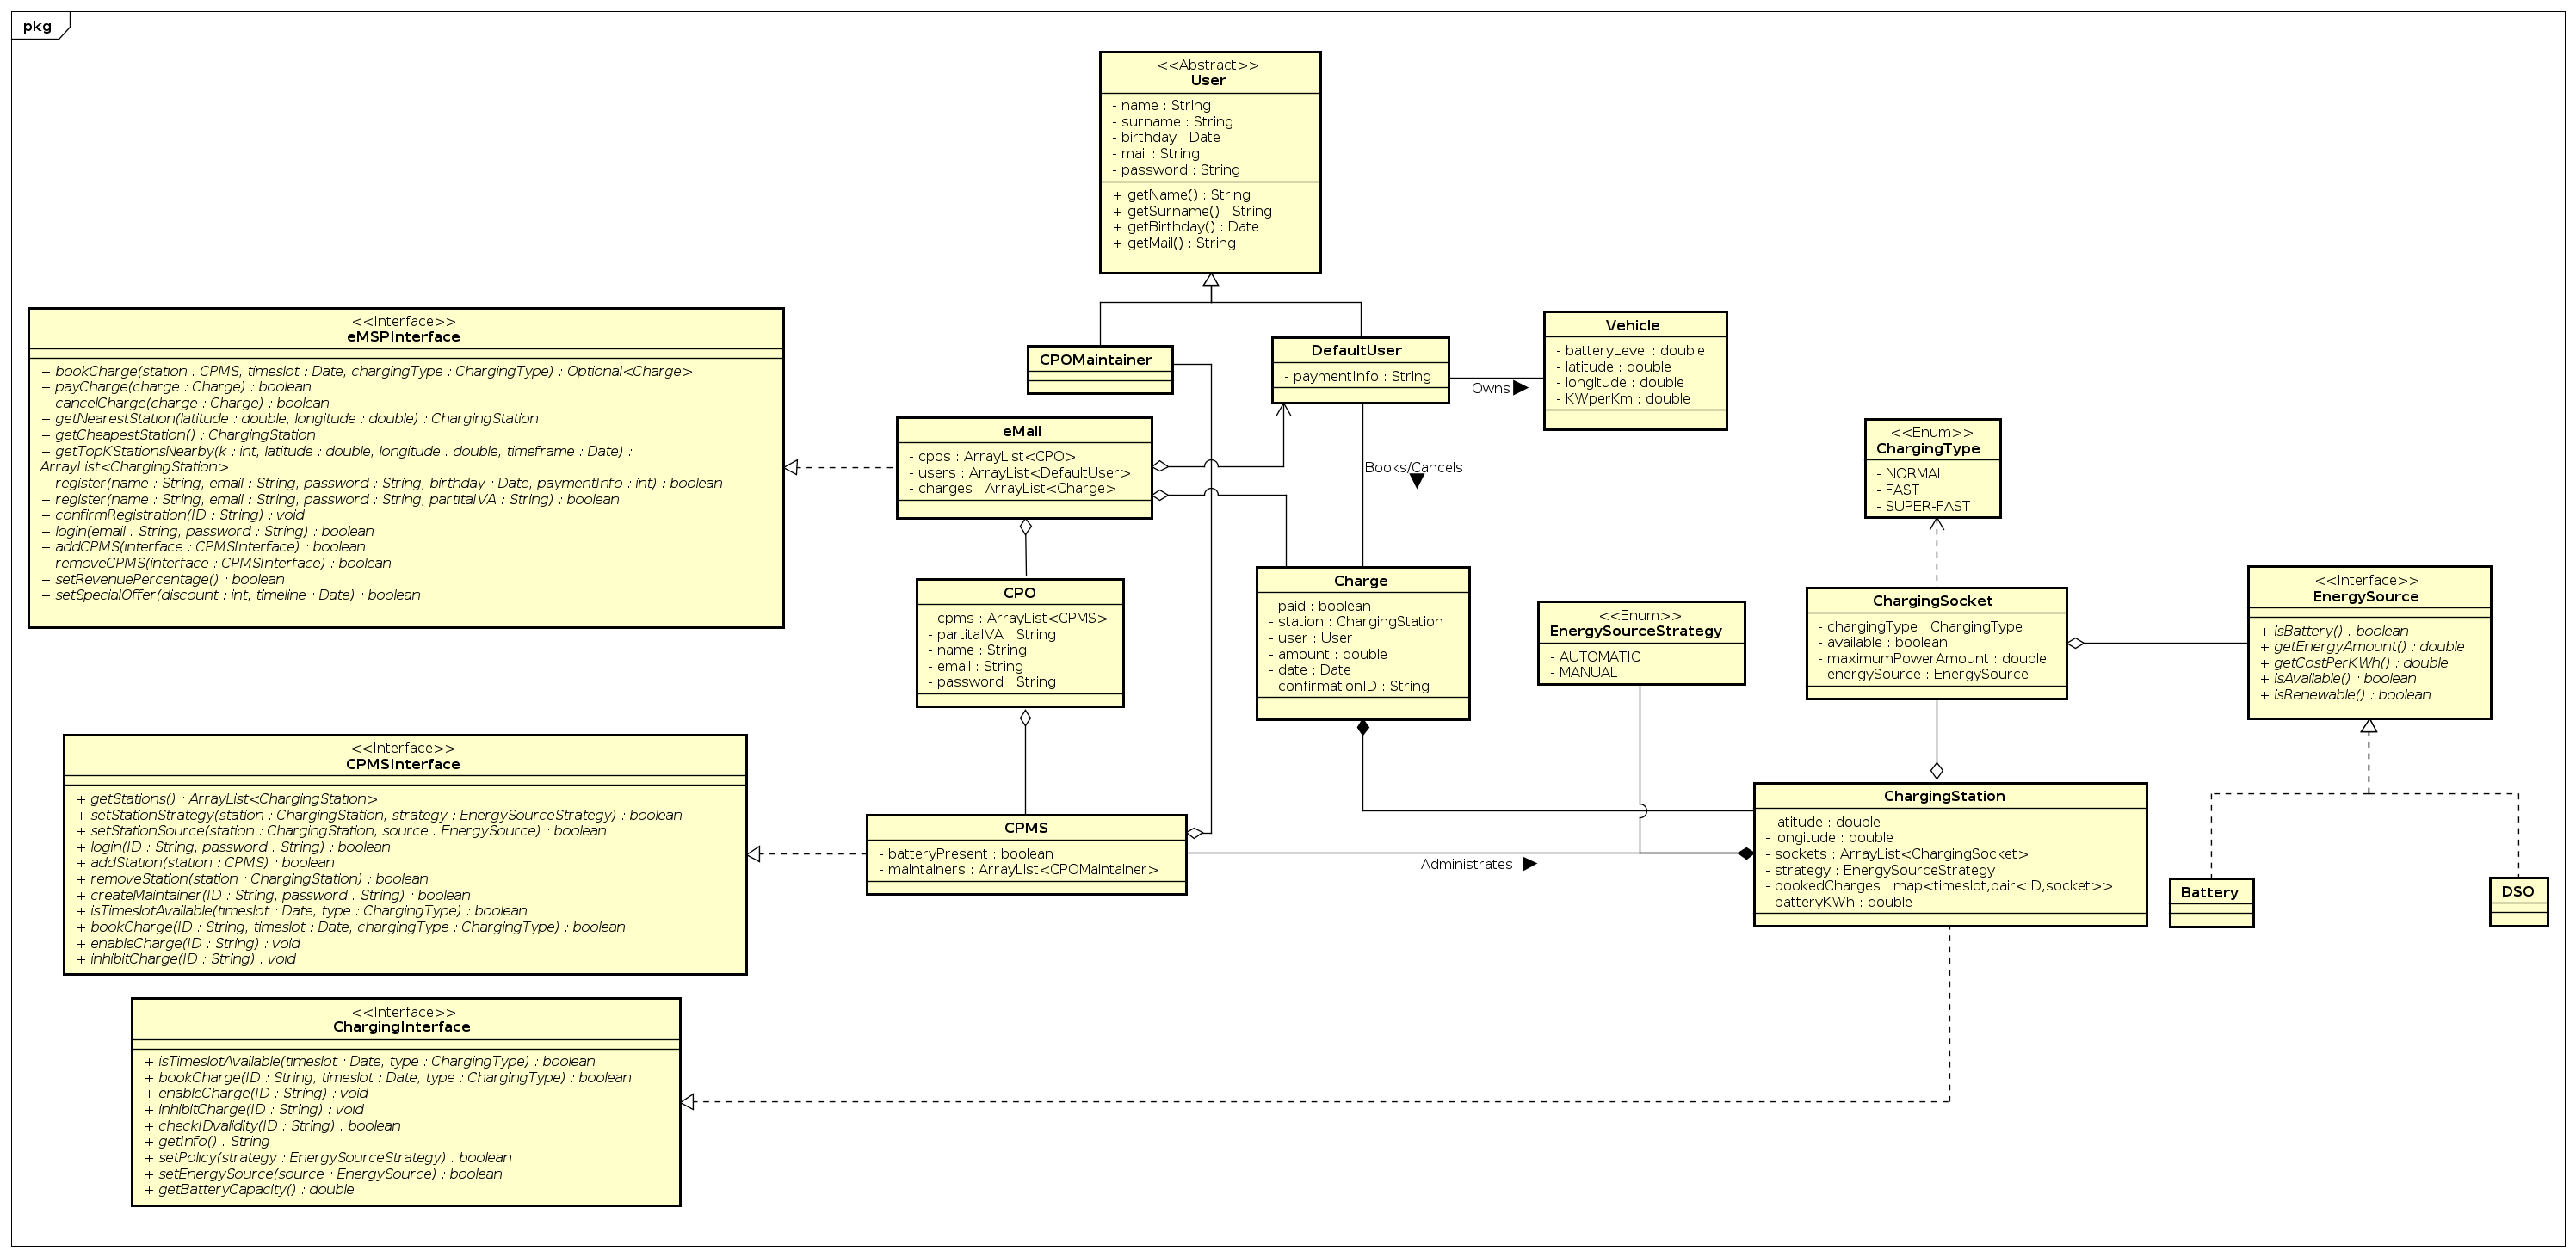
\includegraphics[keepaspectratio, width=16cm]{UML.png}
            \caption{UML}
      \end{center}
\end{figure}
\subsubsection{State diagrams}
\begin{figure}[h!]
      \begin{center}
            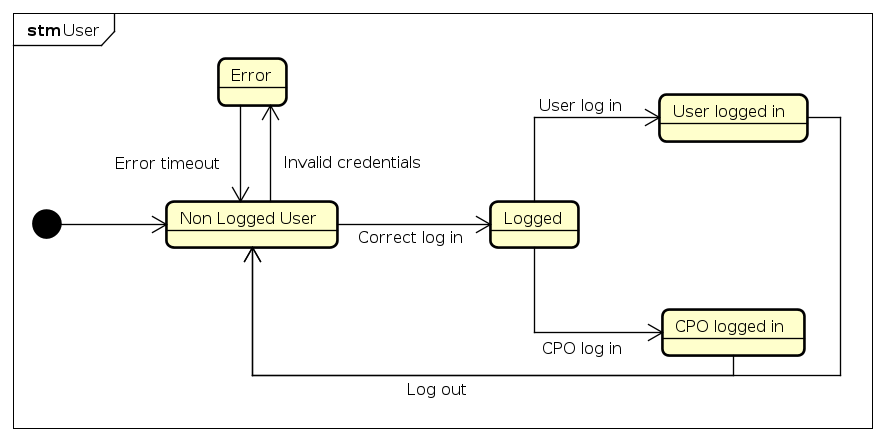
\includegraphics[keepaspectratio, width=16cm]{StateDiagrams/User.png}
            \caption{User state diagram}
      \end{center}
\end{figure}
\begin{figure}[h!]
      \begin{center}
            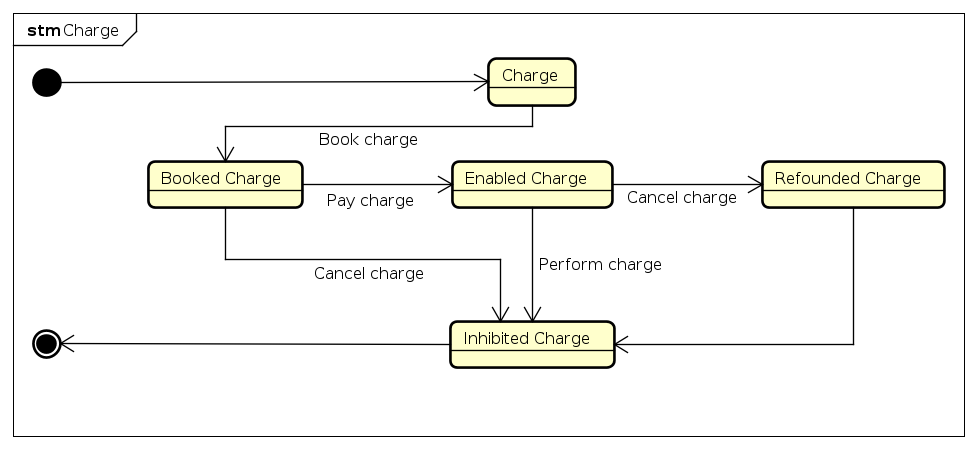
\includegraphics[keepaspectratio, width=16cm]{StateDiagrams/Charge.png}
            \caption{Charge state diagram}
      \end{center}
\end{figure}
\begin{figure}[h!]
      \begin{center}
            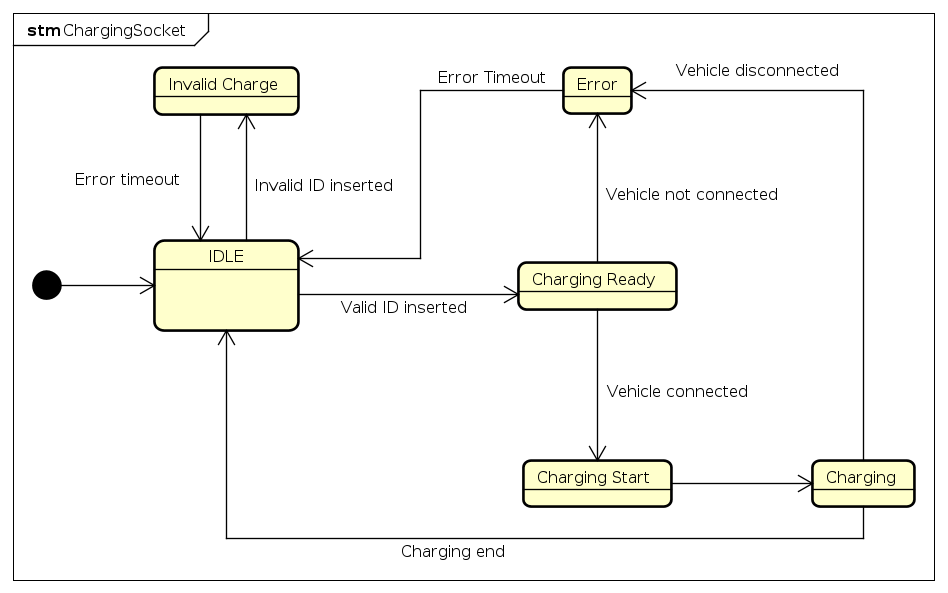
\includegraphics[keepaspectratio, width=16cm]{StateDiagrams/ChargingSocket.png}
            \caption{Charging socket state diagram}
      \end{center}
\end{figure}
\clearpage

\subsection{Product functions}
In the following subsections the functions of each subsystem are described.

\subsubsection{\acf{eMall}}
\paragraph{Accessing the \ac{eMall}}
In order to access the system features an authentication is required. When registering it's mandatory for users to insert Name, Surname, birthday, e-Mail, Password and a Payment Method whereas for \acp{CPO} the required information are Name, e-Mail, Password and \gls{partita IVA}. For the login, an authentication with e-Mail and password is required.

\paragraph{Performing a charge}
The main feature of the system is to help people booking a charge efficiently. The system allows people to see the availability of charging stations and choose where and when to charge the vehicle.
If a user changes his mind, he can delete a previously booked charge.
When the user arrives to the booked socket, he has to insert the confirmation pin in order to start the charging process.
The system notifies the user when the charging process is completed.

\paragraph{Showing information about charging stations}
Whenever a user selects a charging station, location, price, a parameter on how green the energy provided is, special offers and availability of sockets in the station are shown.

\paragraph{Suggesting recharge of the vehicle}
The system offers proactive suggestions about the vehicle recharge via the connection between the vehicle, the electronic calendar and \ac{eMall}. It is able to suggest the user when and where to charge the vehicle to minimize the cost, the environment impact, and the distance from the scheduled appointments.

\subsubsection{\acf{CPMS}}
\paragraph{Accessing the \ac{CPMS}}
In order to manage the \ac{CPMS} an authentication with proper authorization is required. So a \acp{CPO}maintainer can login with ID and password.

\paragraph{Managing the energy source for a charging station}
An authorized \ac{CPO}maintainer can choose manually the energy source (battery or \ac{DSO}) for each station.
Thus a \acp{CPO}maintainer can decide the revenue percentage of a charge and create special offers to increase visibility of the station or to promote greener solutions. If the \ac{CPO}maintainer wishes, the \ac{CPMS} can also work in automatic mode, so the system is able to make all the decisions autonomously.


\subsection{User characteristics}
We consider the following actors in the \ac{eMall} system:
\begin{enumerate}[label=\textbf{A\arabic*}]
      \item \textbf{Unregistered user:} A user that needs to register before accessing the \ac{eMall} services for users;
      \item \textbf{Registered user:} A user that has access to all the \ac{eMall} features.
            This actor can be associated to an electric vehicle and can visualize the nearest stations, book/cancel/pay a charge, visualize the status of a charge and activate the automatic suggestion service based on the agenda;
      \item \textbf{Unregistered \ac{CPO}} A \ac{CPO} that needs to register before accessing the \ac{eMall} services for \acp{CPO};
      \item \textbf{Registered \ac{CPO}} A \ac{CPO} that can add/remove to \ac{eMall} \acp{CPMS};
      \item \textbf{Registered \ac{CPO}maintainer:} A user that has access to all the \ac{CPMS} features. These \ac{CPMS} allows the maintainer to configure the energy source strategy, add other \ac{CPO} maintainers and to visualize all the charging stations statuses;
\end{enumerate}

\subsection{Assumptions and constraints}
\subsubsection{Assumptions}
\begin{enumerate}[label=\textbf{DA\arabic*}]
      \item Users insert genuine data in the forms;
      \item Users (Including \acp{CPO}) do not use the system with malicious intent;
      \item All the electric vehicles can be charged by all the stations (no incompatibility);
      \item All the users have an active internet and GPS connection always available while using the service;
      \item Once installed, the initial login to a \ac{CPMS} is done using the default user and password and the first \ac{CPO}maintainer is configured;
      \item Charging sockets have internet connection and an appropriate interface;
      \item Charging sockets have an input method for inserting the pin so that the user can validate the charge;
      \item The software utilizes payment \acp{API};
\end{enumerate}

\subsubsection{Constraint}
\begin{enumerate}[label=\textbf{C\arabic*}]
      \item If a User wants to use a charging station he must have booked and paid a charge through the system;
      \item If a User wants to change the time slot of a charge he is required to cancel and re-book the charge;
\end{enumerate}

\clearpage